\section{HV-modellen}
\label{apx:hv-modellen}
Vi anvender her HV-Modellen til at gå i dybden med Subscription-Fatigue 

\textbf{Hvad?} 

\begin{itemize}
\item Hvad skal man gøre? 
\item Subscription-Fatigue, primært hvis du bliver udsat for subscription-fatigue, er de hyppigste løsninger at lave en list og danne overvejelser over hvilket du bruger og hvilket du ikke bruger. 
\item Hvad bliver gjort? 
\item Mange bliver bare ved med at betale for deres abonnementer, og kigger ikke efter billigere løsninger, som medfører til et økonomisk tab 
\item Hvad burde blive gjort? 
\item Der burde blive undersøgt efter troværdighed på firmaet du har et abonnement på, herefter undersøg hvor vidt det indeholder hvad du skal bruge, og hvad du ikke bruger. 
\item Undersøg hvordan du også kan finde billigere alternativer til hvad du har abonnementer indenfor. Da grupperede abonnementer hyppigst er billigere. 
\item Hvad kan ellers gøres? 
\item Opsige abonnementet, hvis det ikke har nogle nyttighed 
\item Hvad burde ellers blive gjort? 
\item Opsætte en fast dag, eks hvert 3 måned hvor du gennemgår dine abonnementer igen, og undersøger sine abonnementer igen. 
\end{itemize}

\textbf{Hvorfor?}
\begin{itemize}
    \item Hvorfor gør han/hun det? 
    \item Subskription fatigue forekommer hyppigst, når vedkommet, ikke holder styr på deres abonnementer og ikke framælder dem når de ikke bruger dem. 
    \item Det bygger så op i økonommien og til sidst kan vedkommet ikke huske hvor de mælder dem fra 
    \item Hvorfor gøre det?     
    \item Personen vælger oftest et abonnement, frem for 1gangs betaling, fordi de virker billigre over den korte periode, men senere hen bliver dyt, ellers ligger det på et punkt hvor individet ikke har 1 gangsbeløbet men har råd til at tage et subsciption hvor du afbetaler over længere perioder. 
\end{itemize}
    
\textbf{Hvem?}
\begin{itemize}
    \item Hvem gør det? 
    \item Det er typisk, ældre puplikum som falder i abonnomenter, som Telefon abonnoment, tv abonnoment, Lån, elregninger, telefon apps. 
    \item Som trækker på din økonomi månedligt. 
\end{itemize}

\textbf{Hvornår?}
\begin{itemize}
    \item Hvornår skal man gøre noget ved det? 
    \item Subscription fatigue skal behandles så snart du kan mærke økonomiske fald, så dine økonomiske tab kan minimeres hurtigst muligt 
    \item Hvornår kan det ellers blive gjort? 
    \item Du kan gøre noget ved det, men hvis du kan få gjort noget ved det hurtigst muligt vil det minimere skaderne. 
\end{itemize}

\begin{landscape}
    \section{Første skitse af applikation}
    \label{apx:dig_skitse_af_app}
    \begin{center}
        \fbox{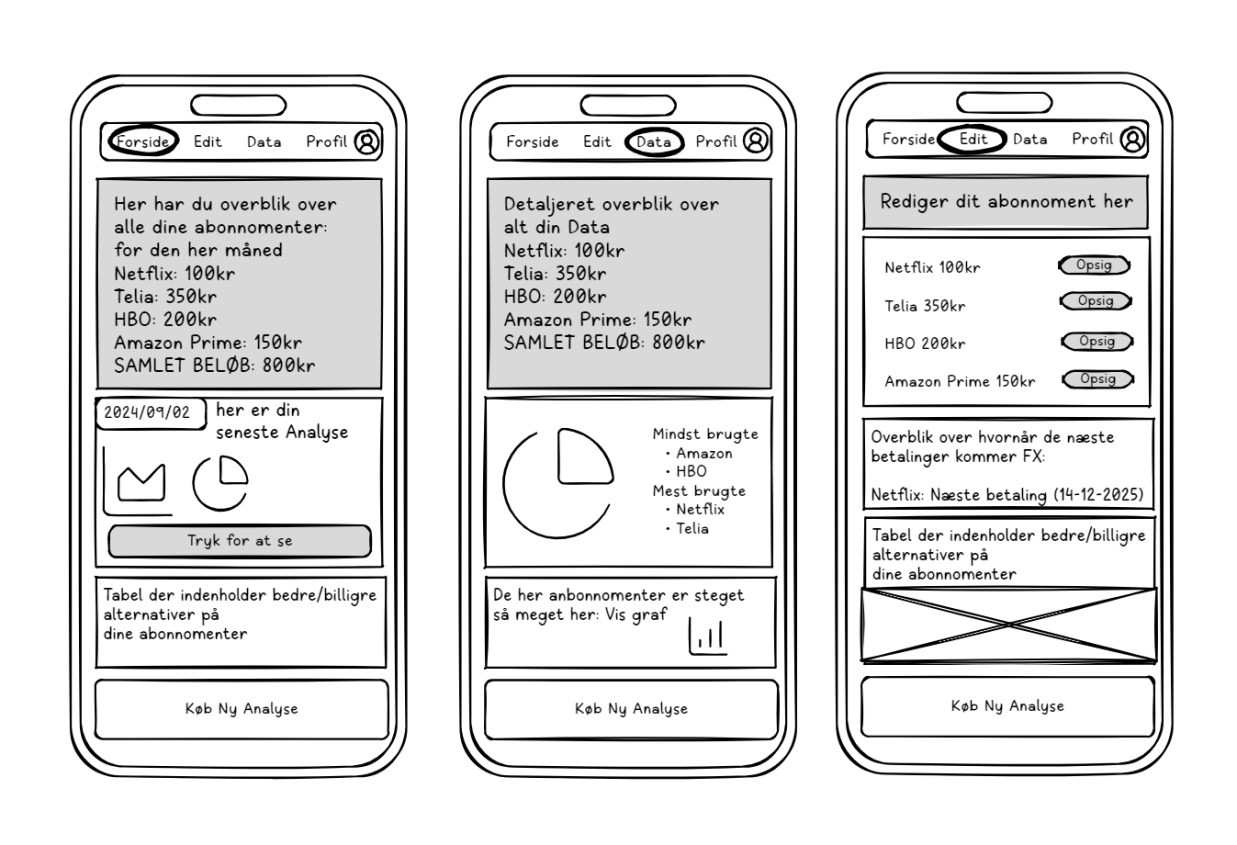
\includegraphics[width=0.8\linewidth]{../latex-document/assets/skitse_af_app.png}}
    \end{center}
\end{landscape}

\newpage

\section{skitse af navbar til a/b test}
\textbf{A version af navigationsbjælken}
  \begin{figure}[H]
    \label{apx:navbar_ab_test}
    \centering
    \fbox{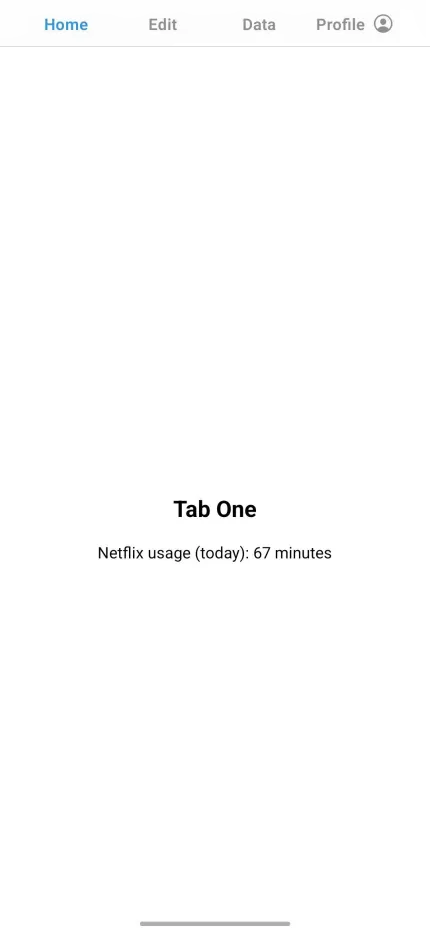
\includegraphics[width=0.5\textwidth]{assets/proto_0001_home.png}}
    \caption{A version af navigationsbjælken}
  \end{figure}

  \textbf{B version af navigationsbjælken}
  \begin{figure}[H]
    \centering
    \fbox{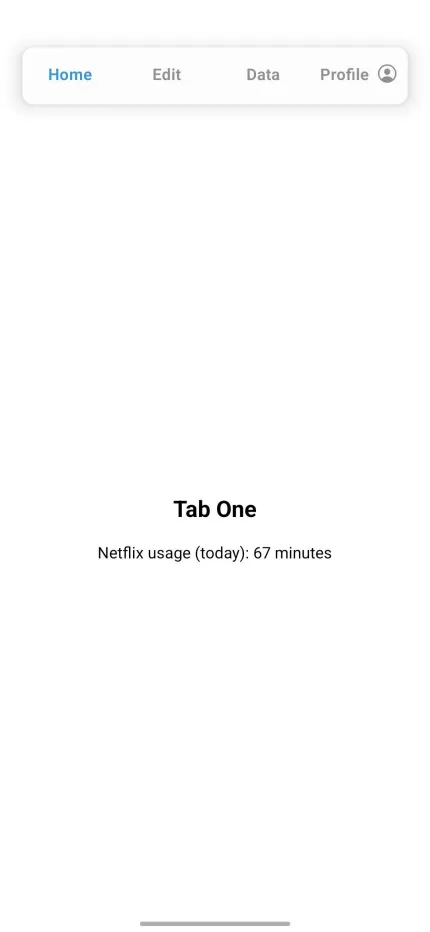
\includegraphics[width=0.5\textwidth]{assets/proto_1_home.png}}
    \caption{B version af navigationsbjælken}
  \end{figure}

\newpage
\section{Skærmbillede af data-side}
\begin{figure}
    \centering
    \fbox{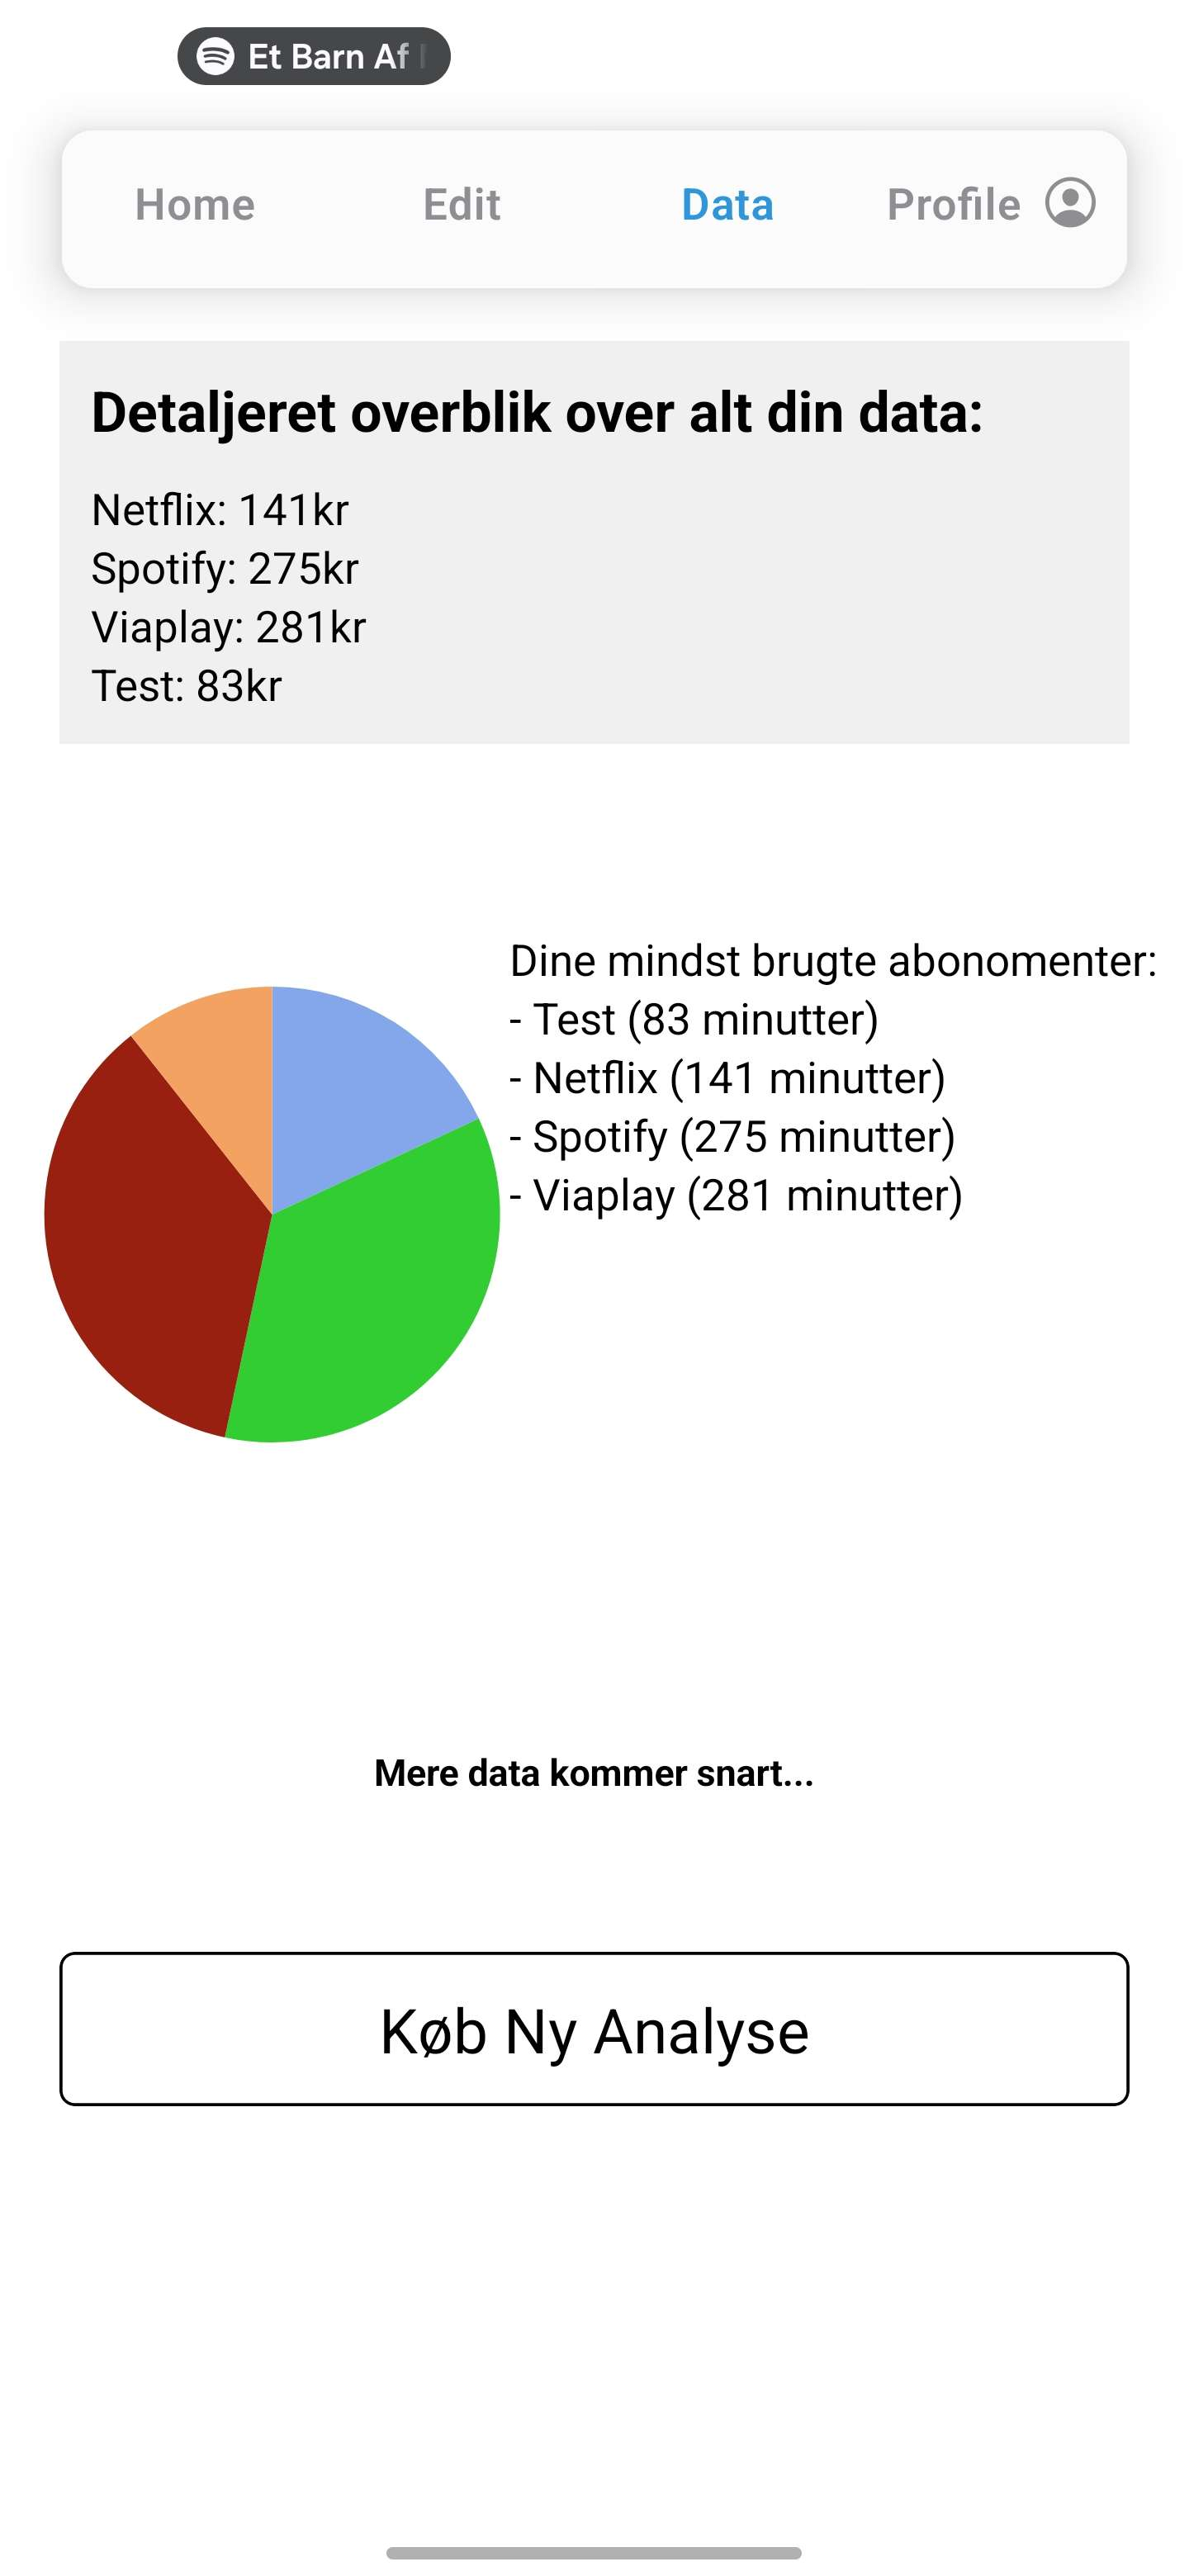
\includegraphics[width=0.5\textwidth]{assets/data_page_graph.jpg}}
    \caption{Skærmbillede af data-side}
\end{figure}

\newpage
\section{Kildekode dataindsamling}
\label{apx:getUsage}
\begin{mdframed}[backgroundcolor=blue!5]
\begin{minted}[breaklines]{tsx}
import * as UsageStats from 'expo-android-usagestats';
import { Alert, Linking, Platform } from 'react-native';


export async function ensureUsagePermission(): Promise<boolean> {
  if (Platform.OS !== 'android') return true;

  try {
    const has = await UsageStats.hasUsageStatsPermission();
    if (has) return true;

    await UsageStats.requestUsageStatsPermission();

    const hasAfter = await UsageStats.hasUsageStatsPermission();
    if (hasAfter) return true;

    Alert.alert(
      'Usage access required',
      'This feature needs Android Usage Access to read app foreground times. Open settings to grant access?',
      [
        { text: 'Cancel', style: 'cancel' },
        {
          text: 'Open Settings',
          onPress: () => {
            Linking.openSettings().catch(() => {});
          },
        },
      ]
    );

    return false;
  } catch (err) {
    console.warn('Error checking/requesting usage permission', err);
    return false;
  }
}


export async function getUsageForPackage(packageName: string, days = 1): Promise<
  { totalTimeInForeground: number; minutes: number } | null
> {
  const end = Date.now();
  const start = end - days * 24 * 60 * 60 * 1000;
  const stats = await UsageStats.getUsageStats(start, end);
  const needle = packageName.toLowerCase();

  const matches = stats.filter((app) => {
    if (!app || !app.packageName) return false;
    const pn = String(app.packageName).toLowerCase();
    const an = String((app as any).appName ?? '').toLowerCase();
    return pn === needle || pn.includes(needle) || an.includes(needle);
  });

  if (!matches || matches.length === 0) {
    console.log(`getUsageForPackage: no usage-stats entries matched '${packageName}' for ${days} day(s). Top packages:`);
    stats.slice(0, 20).forEach((s: any, i: number) => {
      const pn = s.packageName ?? s.package ?? '(unknown)';
      const ms = (s as any).totalTimeInForeground ?? (s as any).totalTimeForeground ?? (s as any).totalForegroundTime ?? (s as any).totalTime ?? 0;
      console.log(i, pn, ms);
    });
    return null;
  }

  const getMs = (s: any) => {
    return (
      s.totalTimeInForeground ??
      s.totalTimeForeground ??
      s.totalForegroundTime ??
      s.totalTime ??
      s.totalTimeForegroundServiceUsed ??
      0
    );
  };

  const totalMs = matches.reduce((acc: number, s: any) => acc + (Number(getMs(s)) || 0), 0);

  if (totalMs === 0) {
    console.log(`getUsageForPackage: matched entries for '${packageName}' but totalMs==0 for ${days} day(s). Matches:`);
    matches.forEach((m: any, i: number) => console.log(i, m.packageName, getMs(m), m));
  }

  const minutes = Math.round(totalMs / 60000);
  return { totalTimeInForeground: totalMs, minutes };
}
\end{minted}
\end{mdframed}

\newpage
\section{Skærmbilleder af produktet}
\begin{landscape}
\begin{figure}
  \fbox{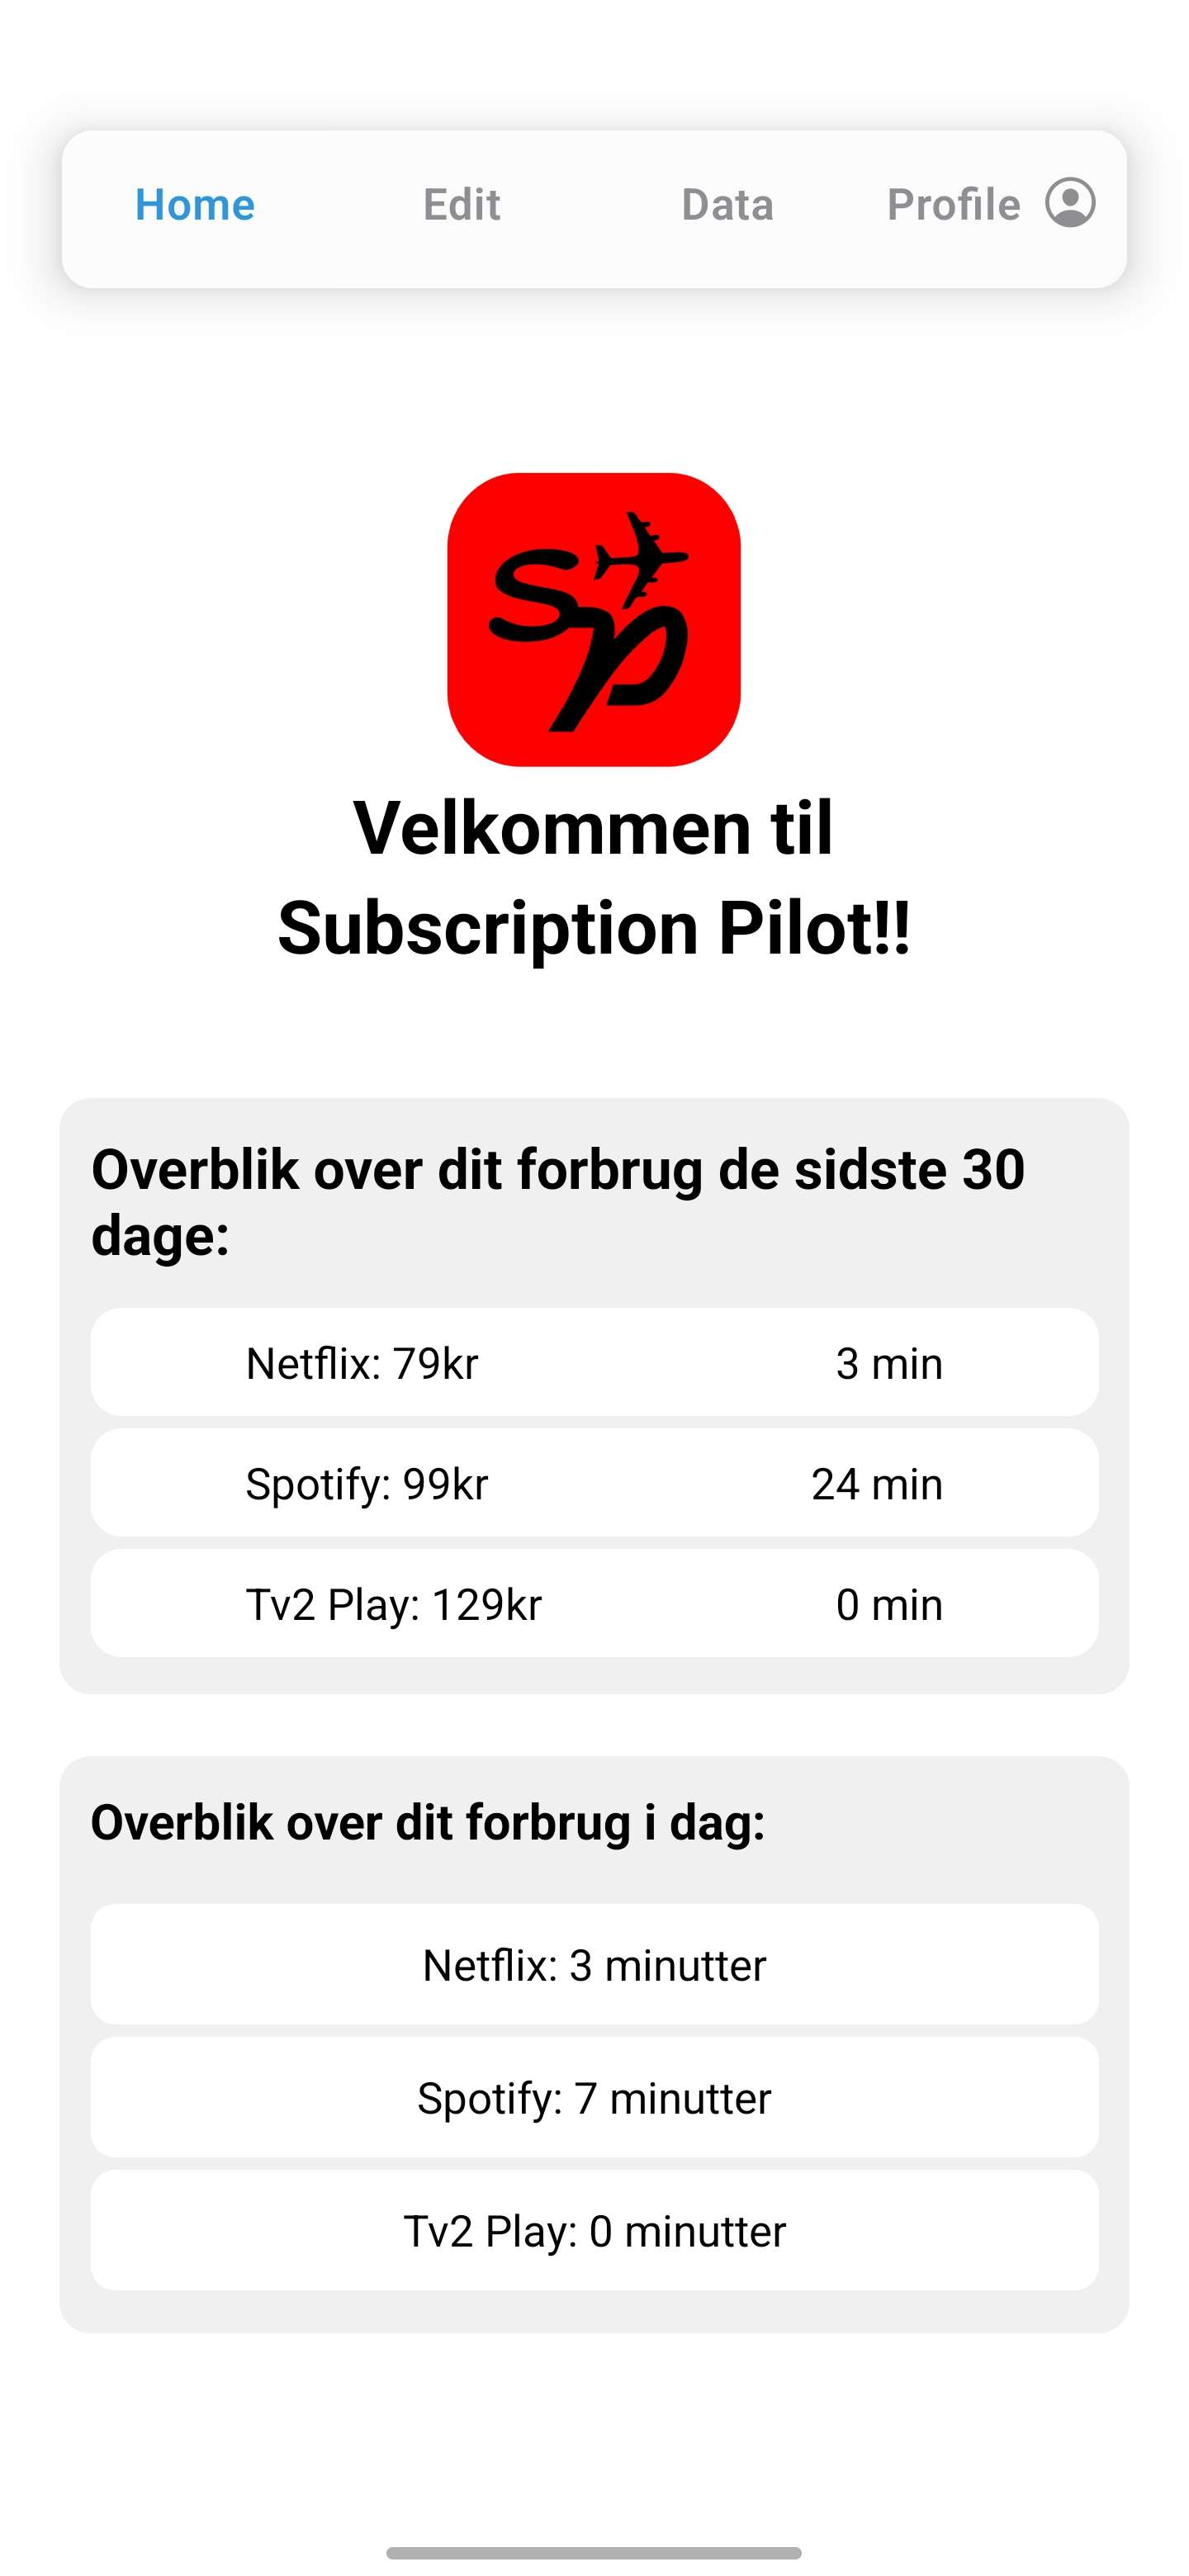
\includegraphics[width=0.5\textwidth]{assets/hifi-skitser/home-before-yt.jpg}}
  \fbox{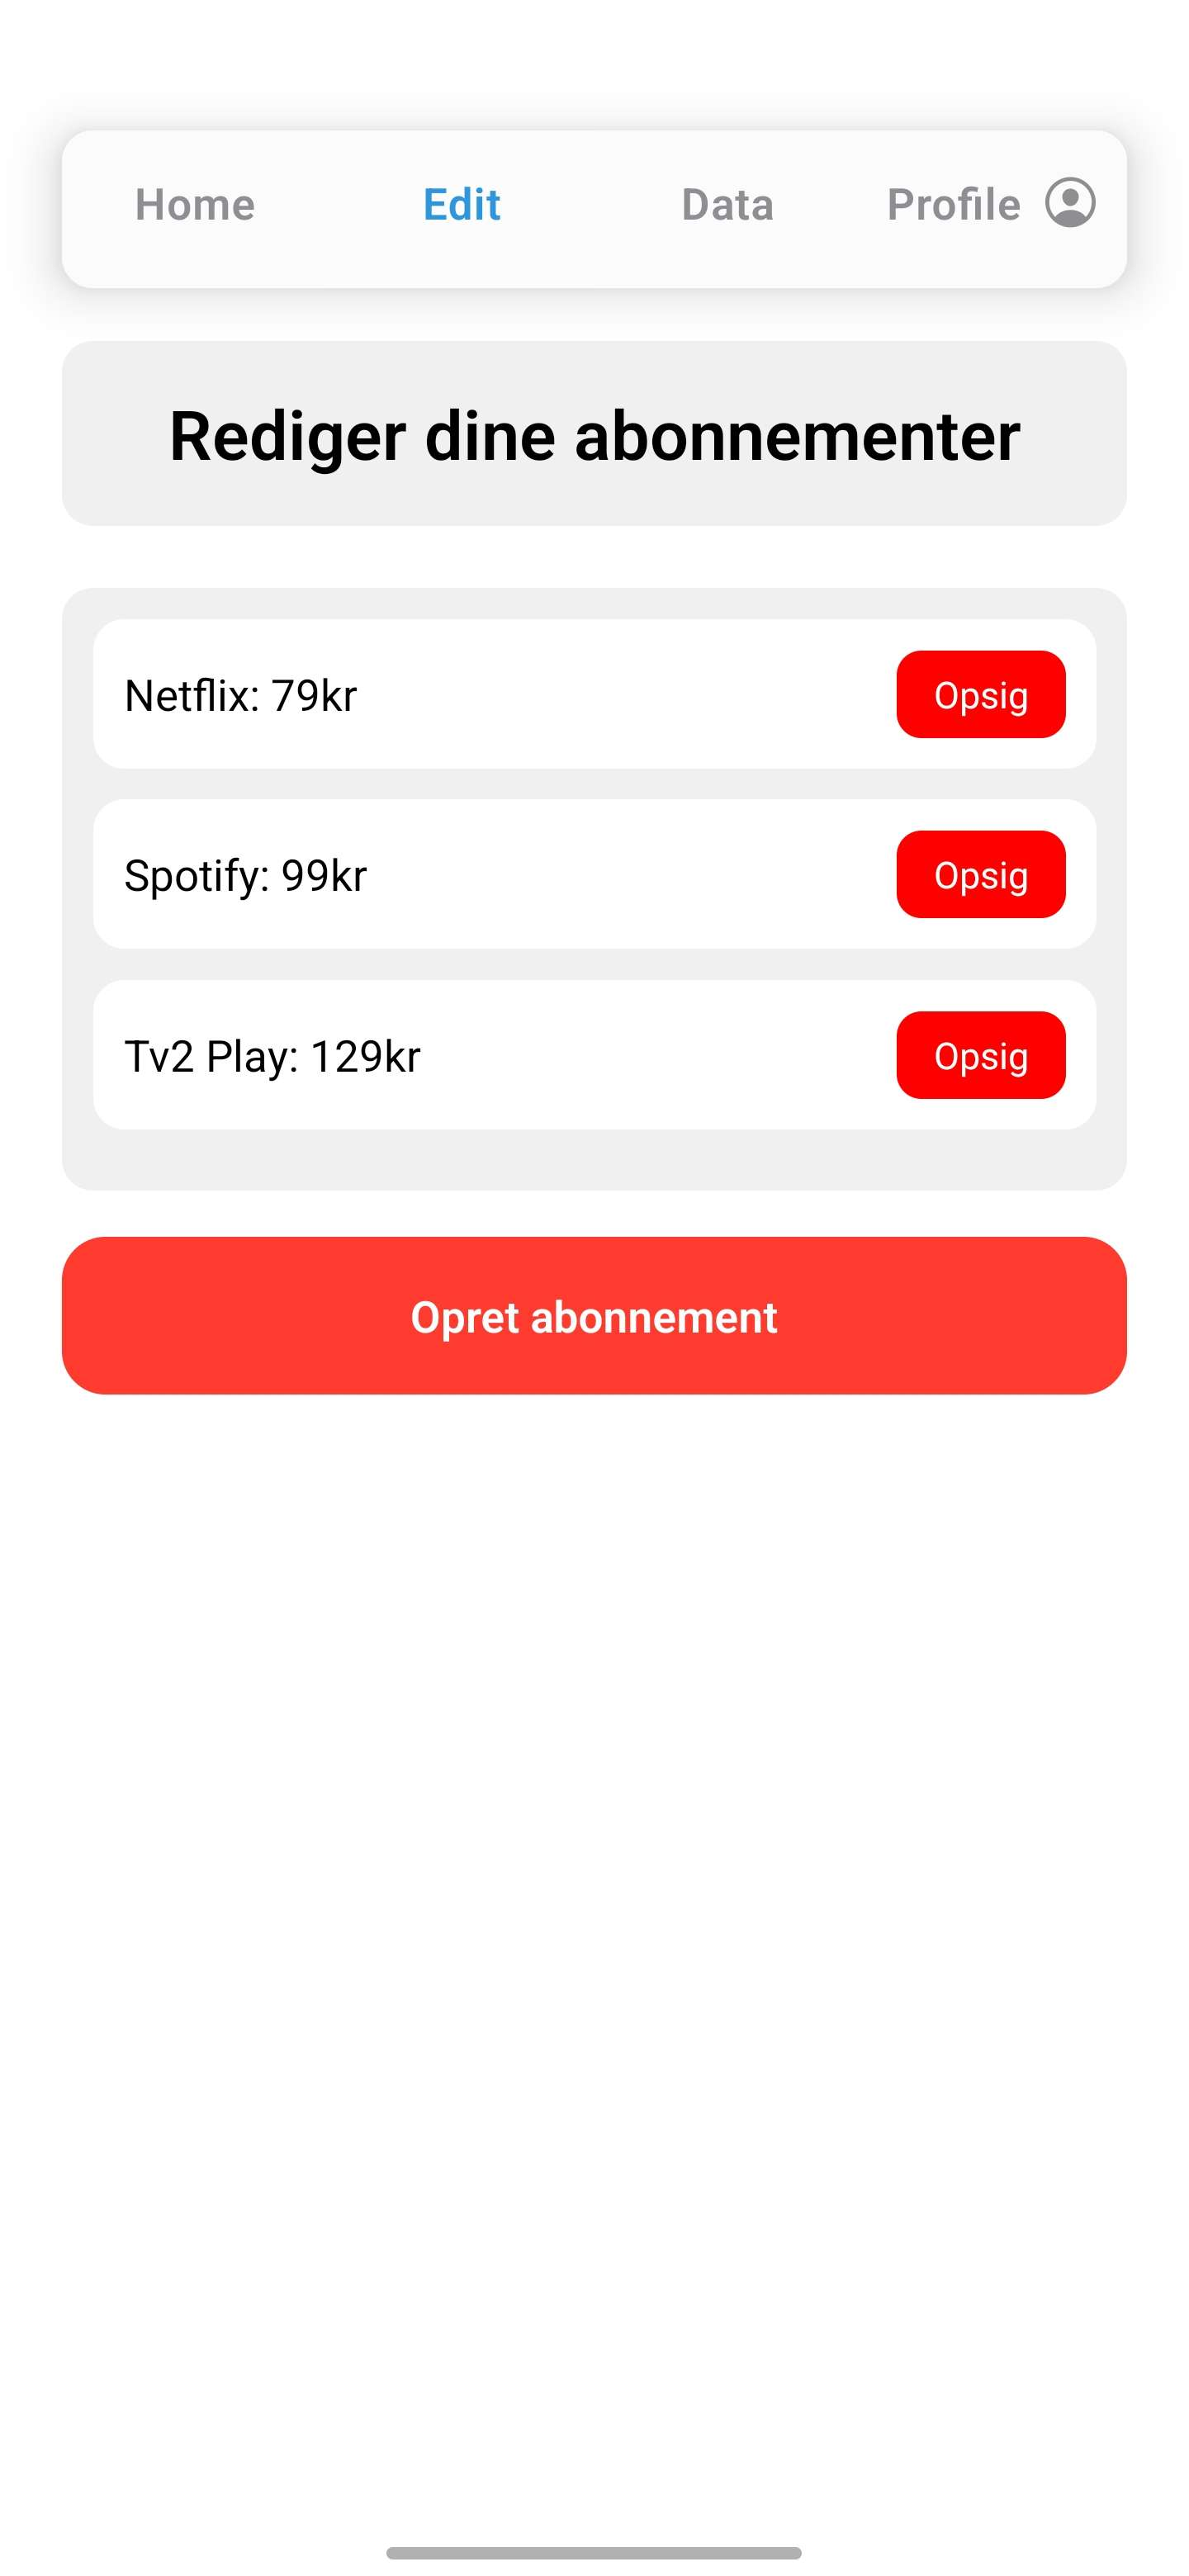
\includegraphics[width=0.5\textwidth]{assets/hifi-skitser/edit_before_yt.jpg}}
  \fbox{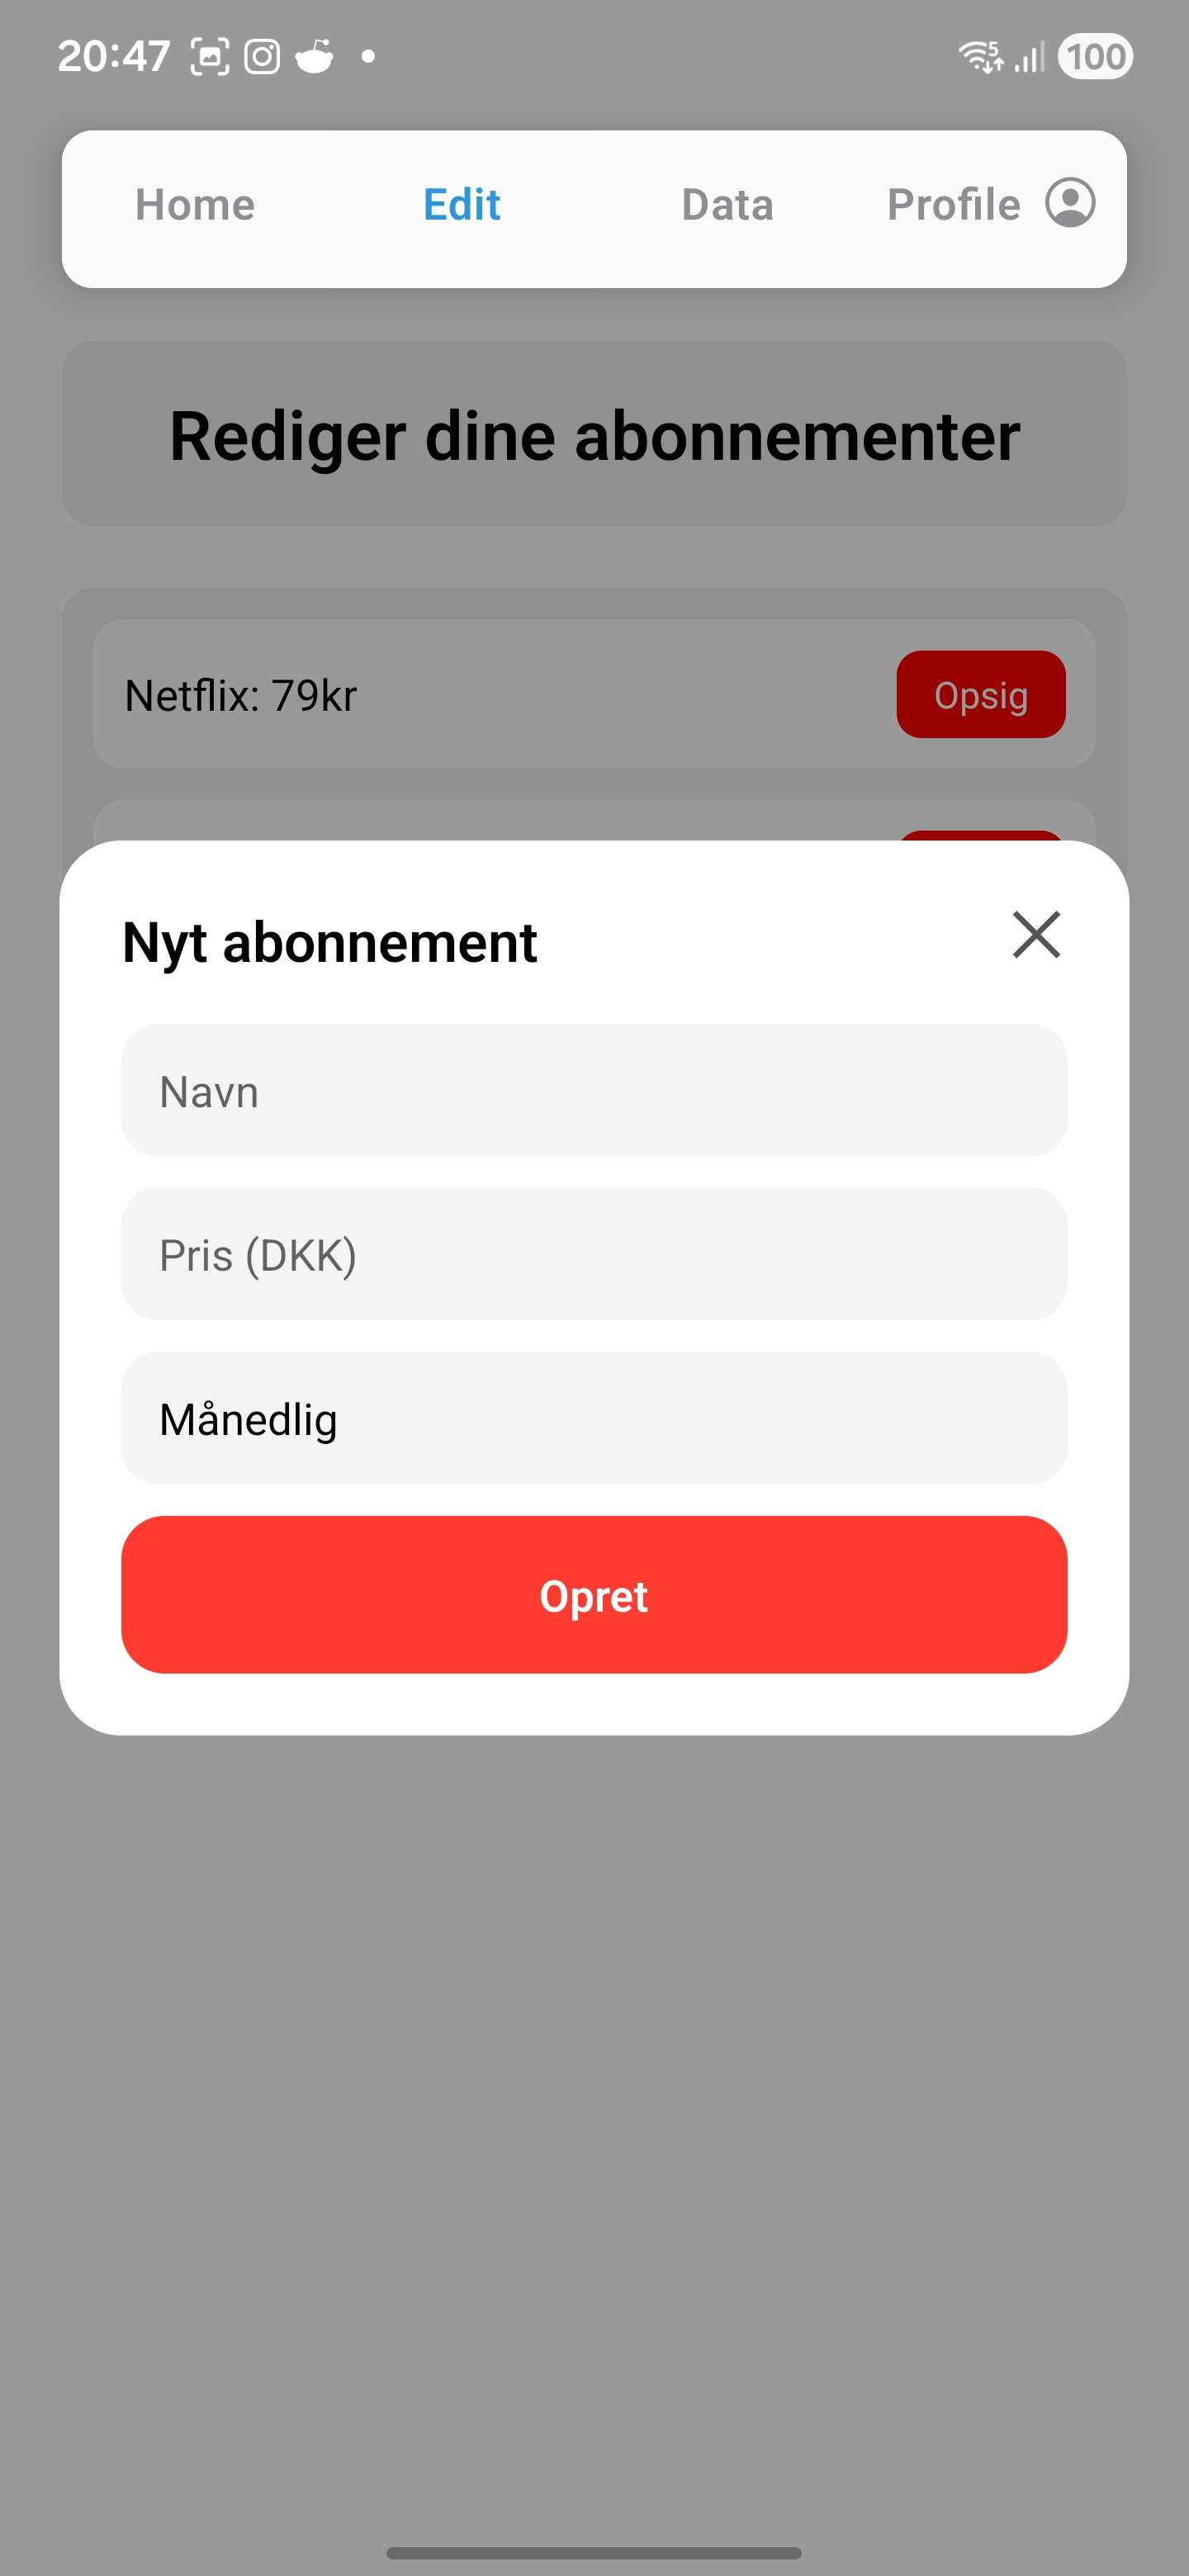
\includegraphics[width=0.5\textwidth]{assets/hifi-skitser/edit-opret.jpg}}
\end{figure}  
\end{landscape}

\begin{landscape}
  \begin{figure}
    \fbox{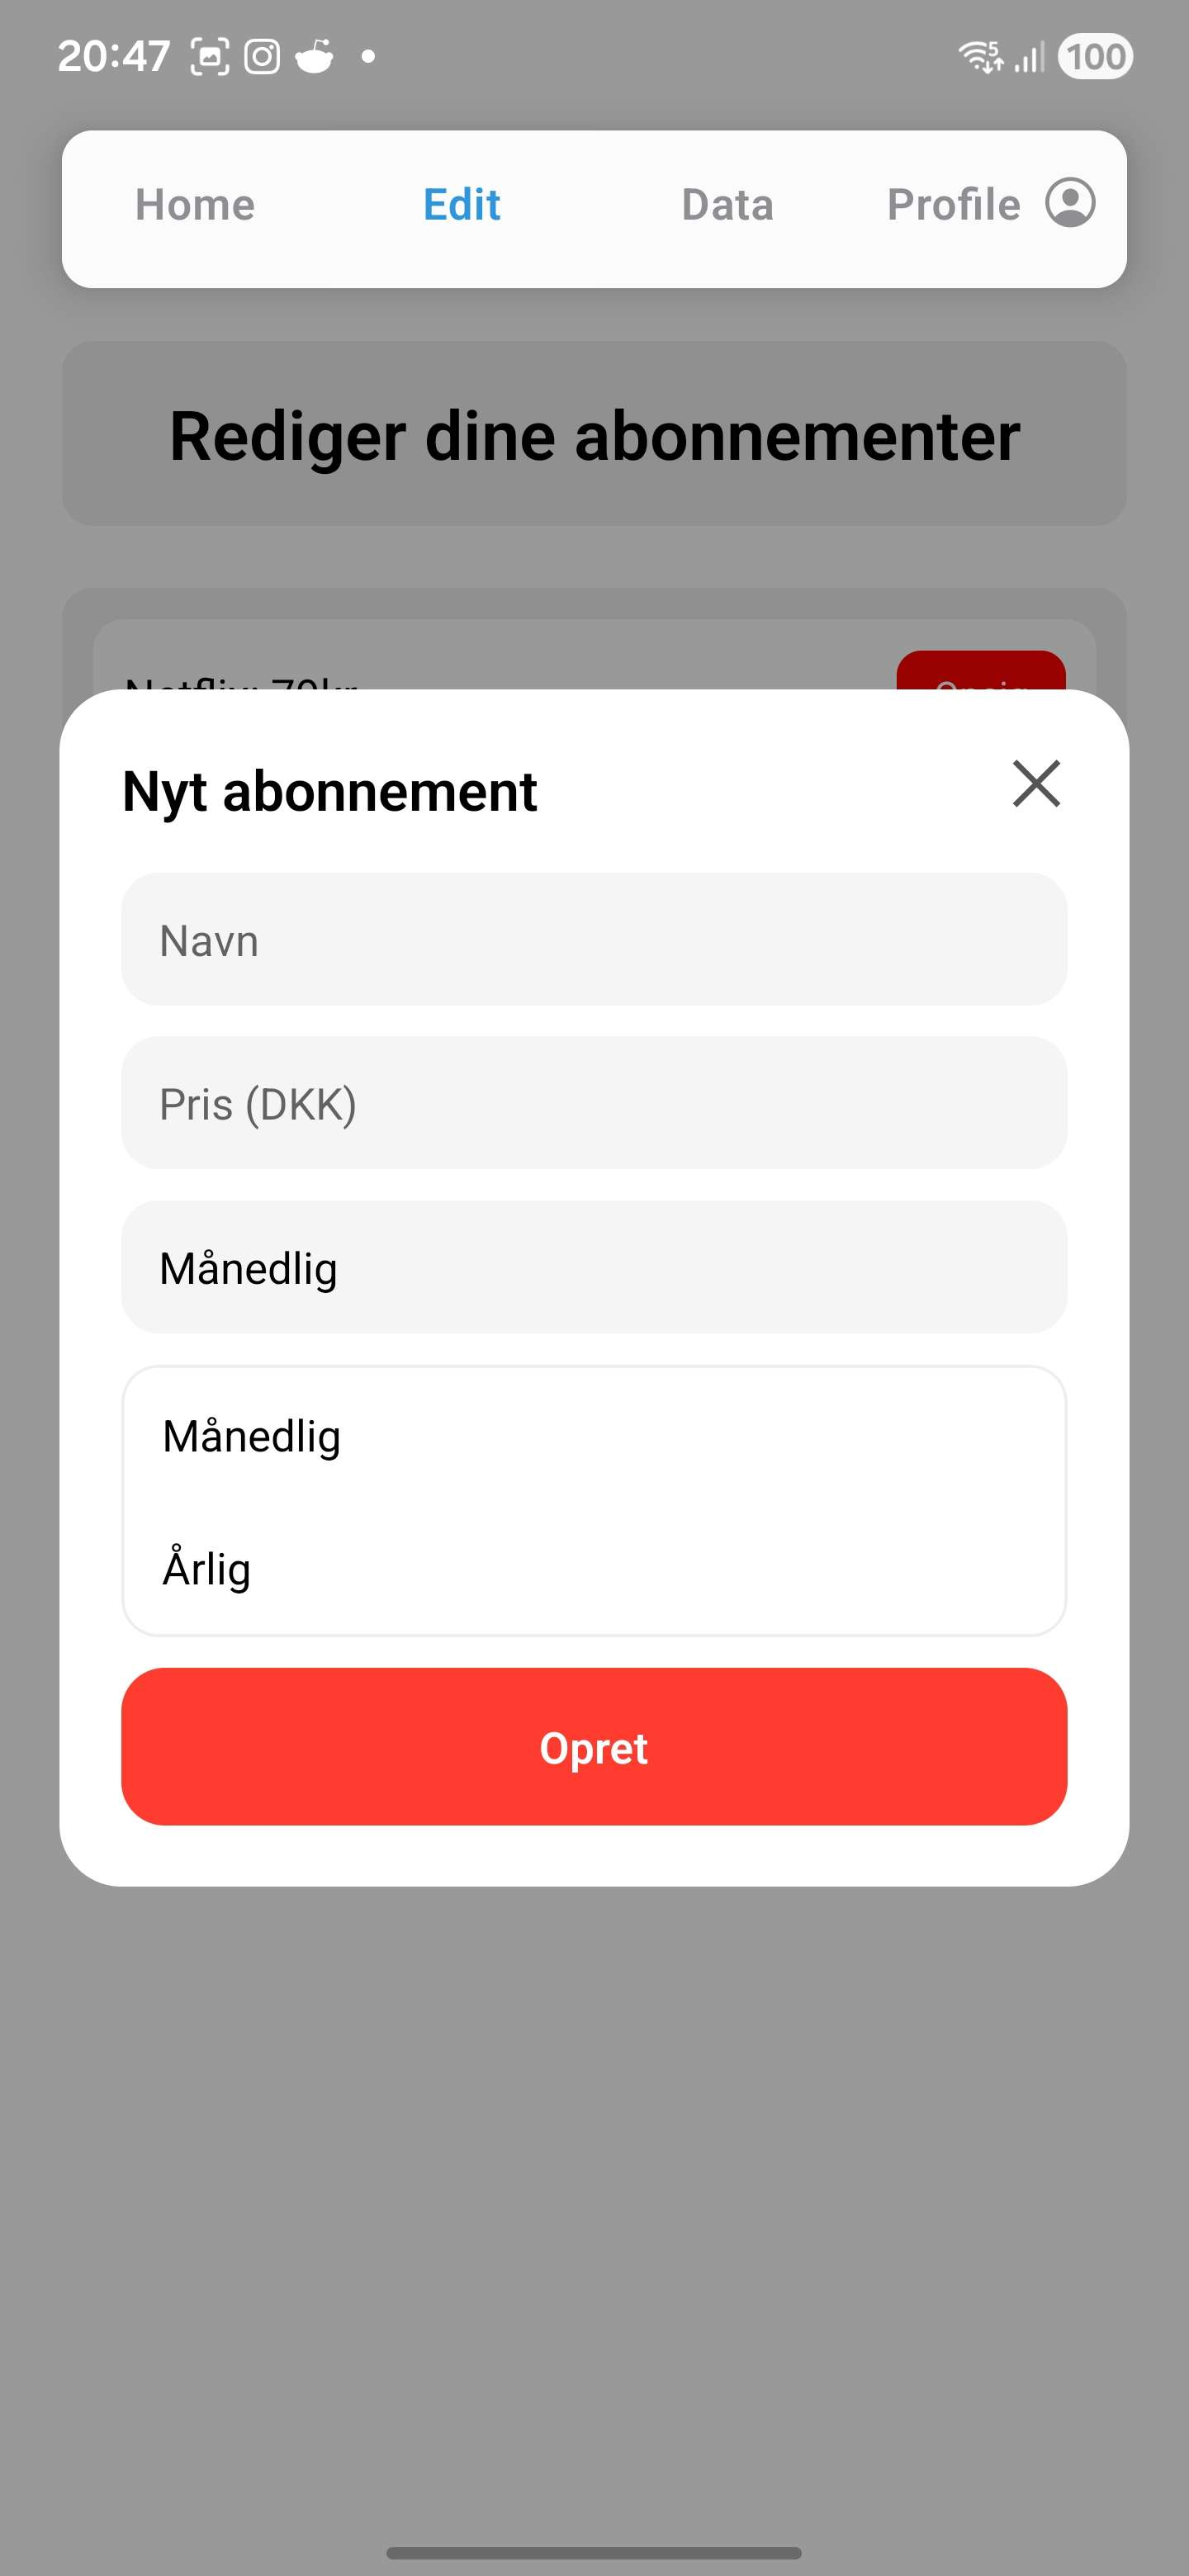
\includegraphics[width=0.5\textwidth]{assets/hifi-skitser/edit-opret-dropdown.jpg}}
    \fbox{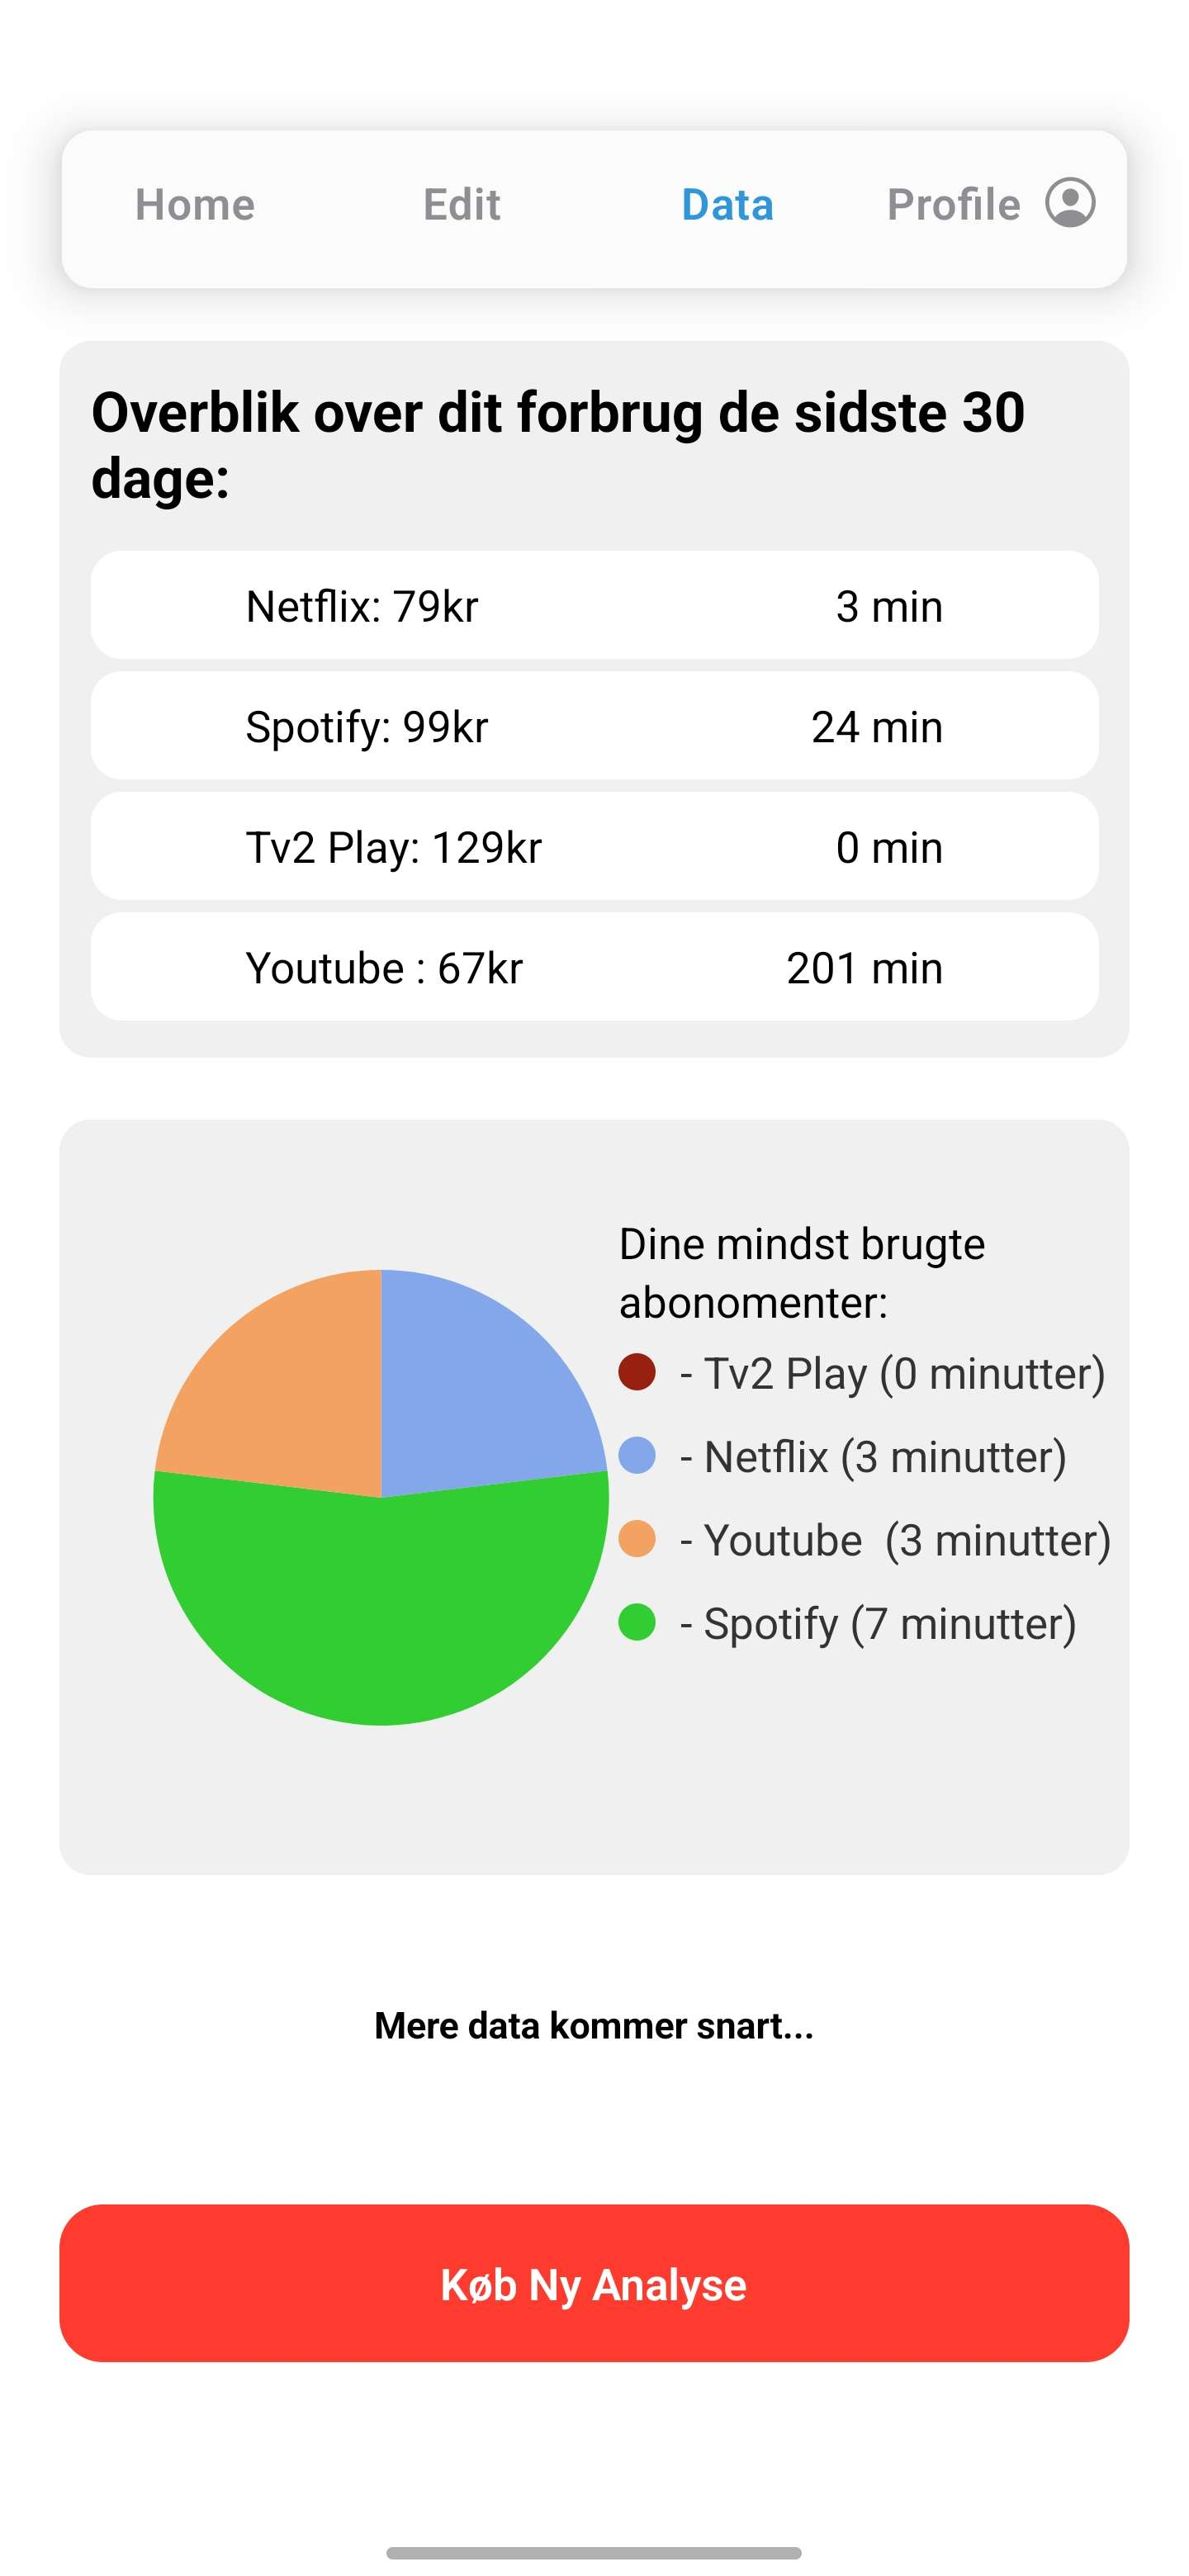
\includegraphics[width=0.5\textwidth]{assets/hifi-skitser/data-after-yt.jpg}}
    \fbox{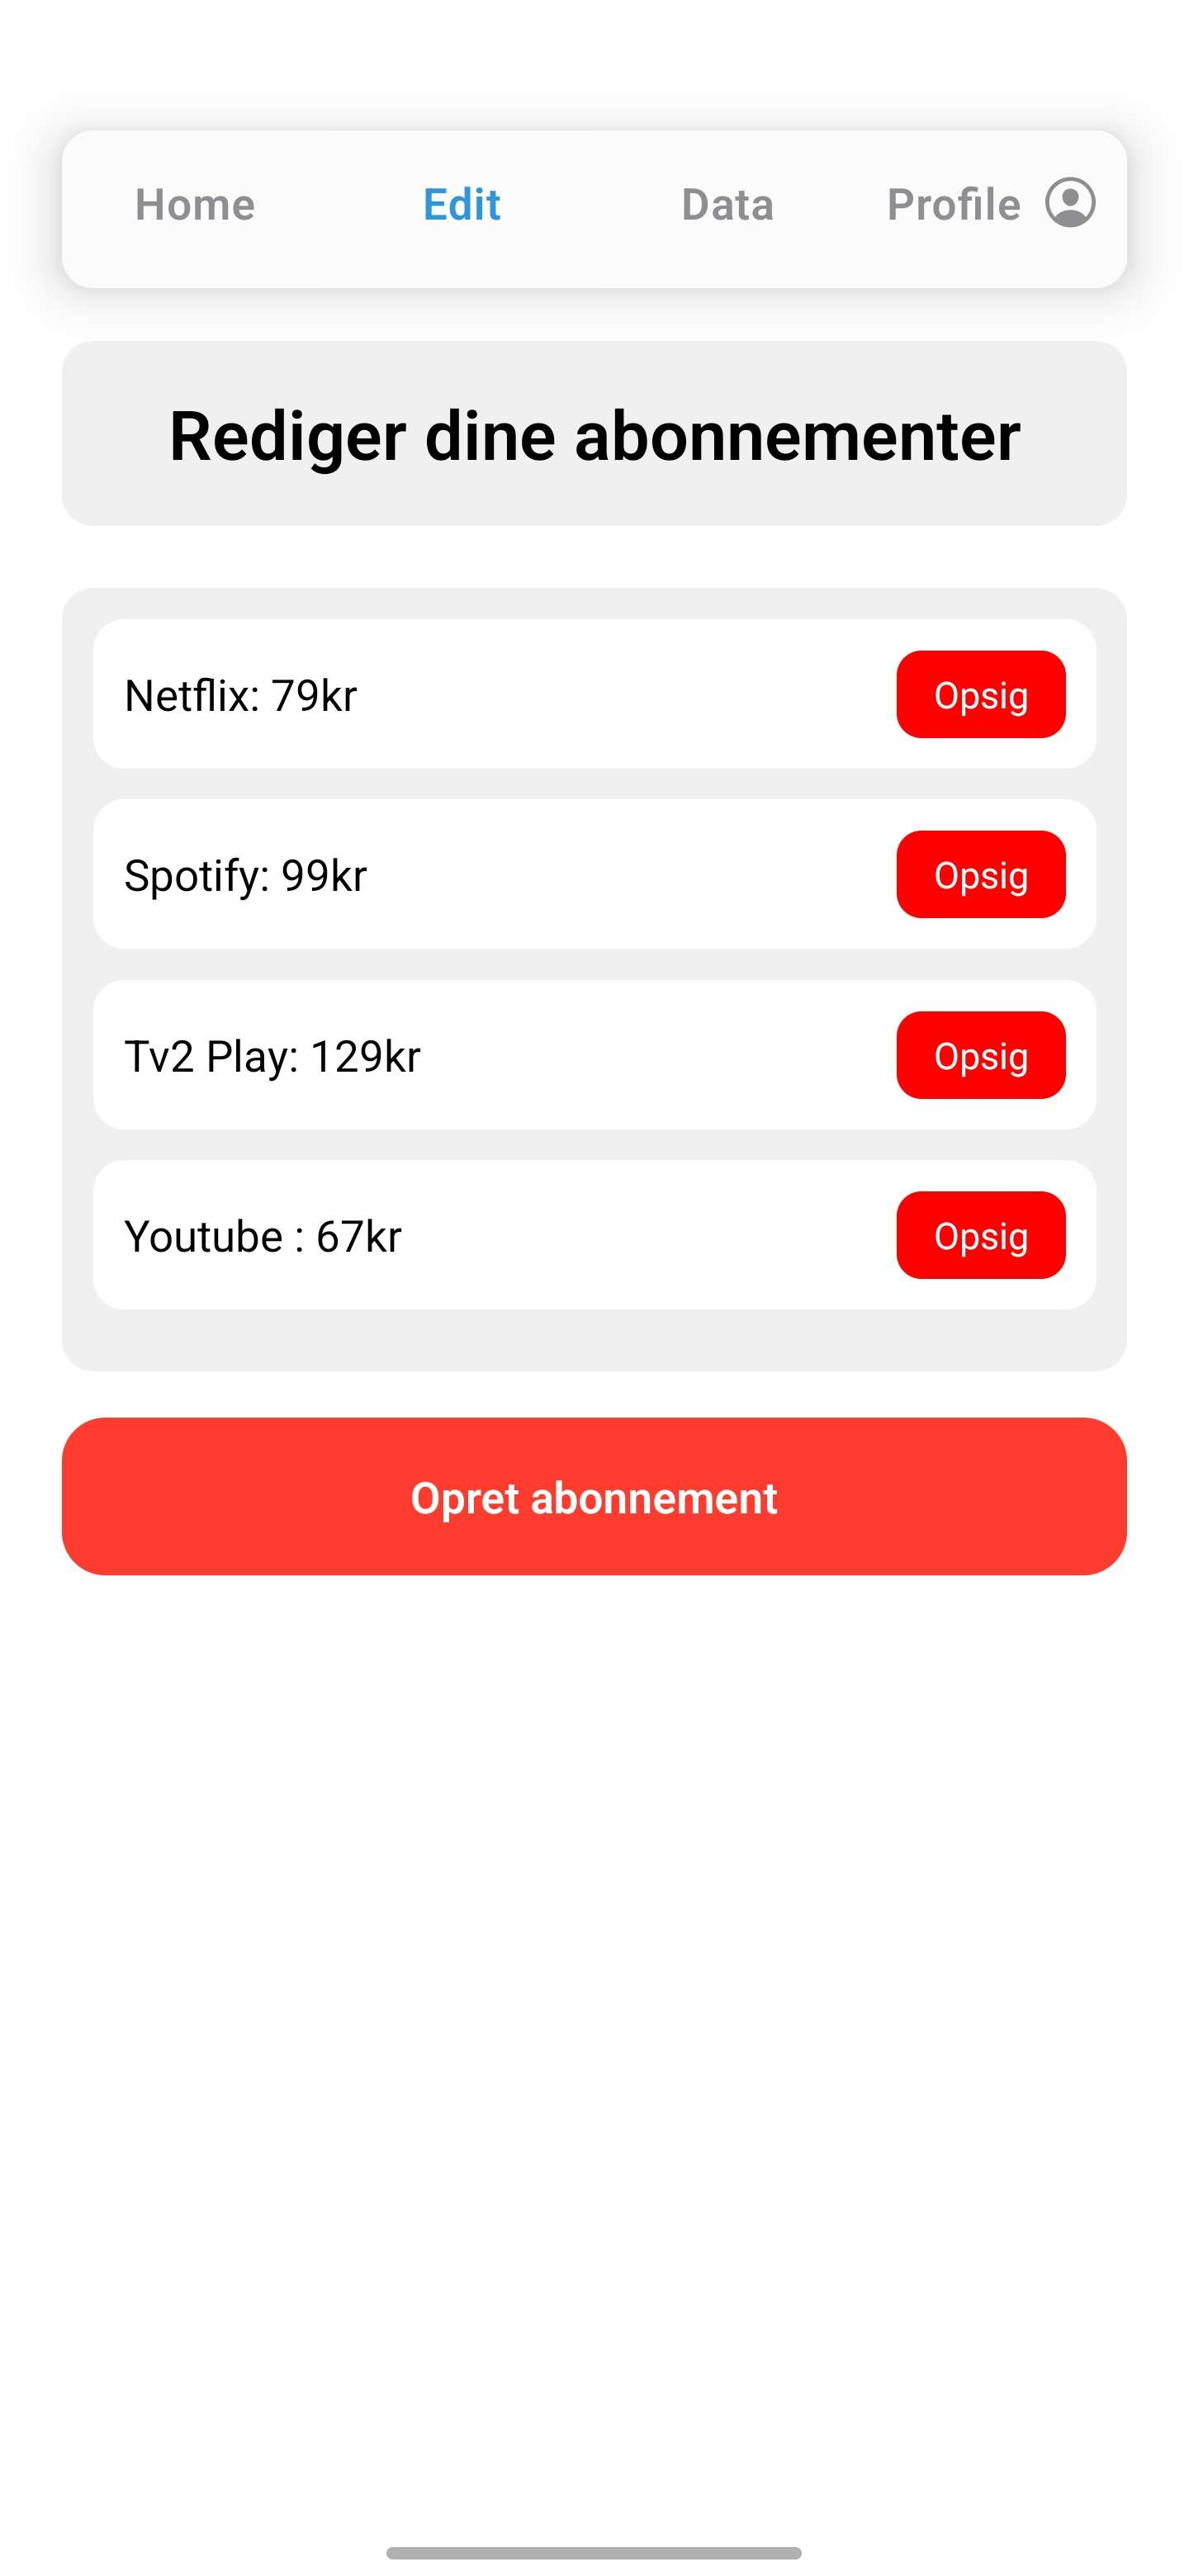
\includegraphics[width=0.5\textwidth]{assets/hifi-skitser/edit.jpg}}
  \end{figure}
\end{landscape}
\begin{landscape}
  \begin{figure}
    \fbox{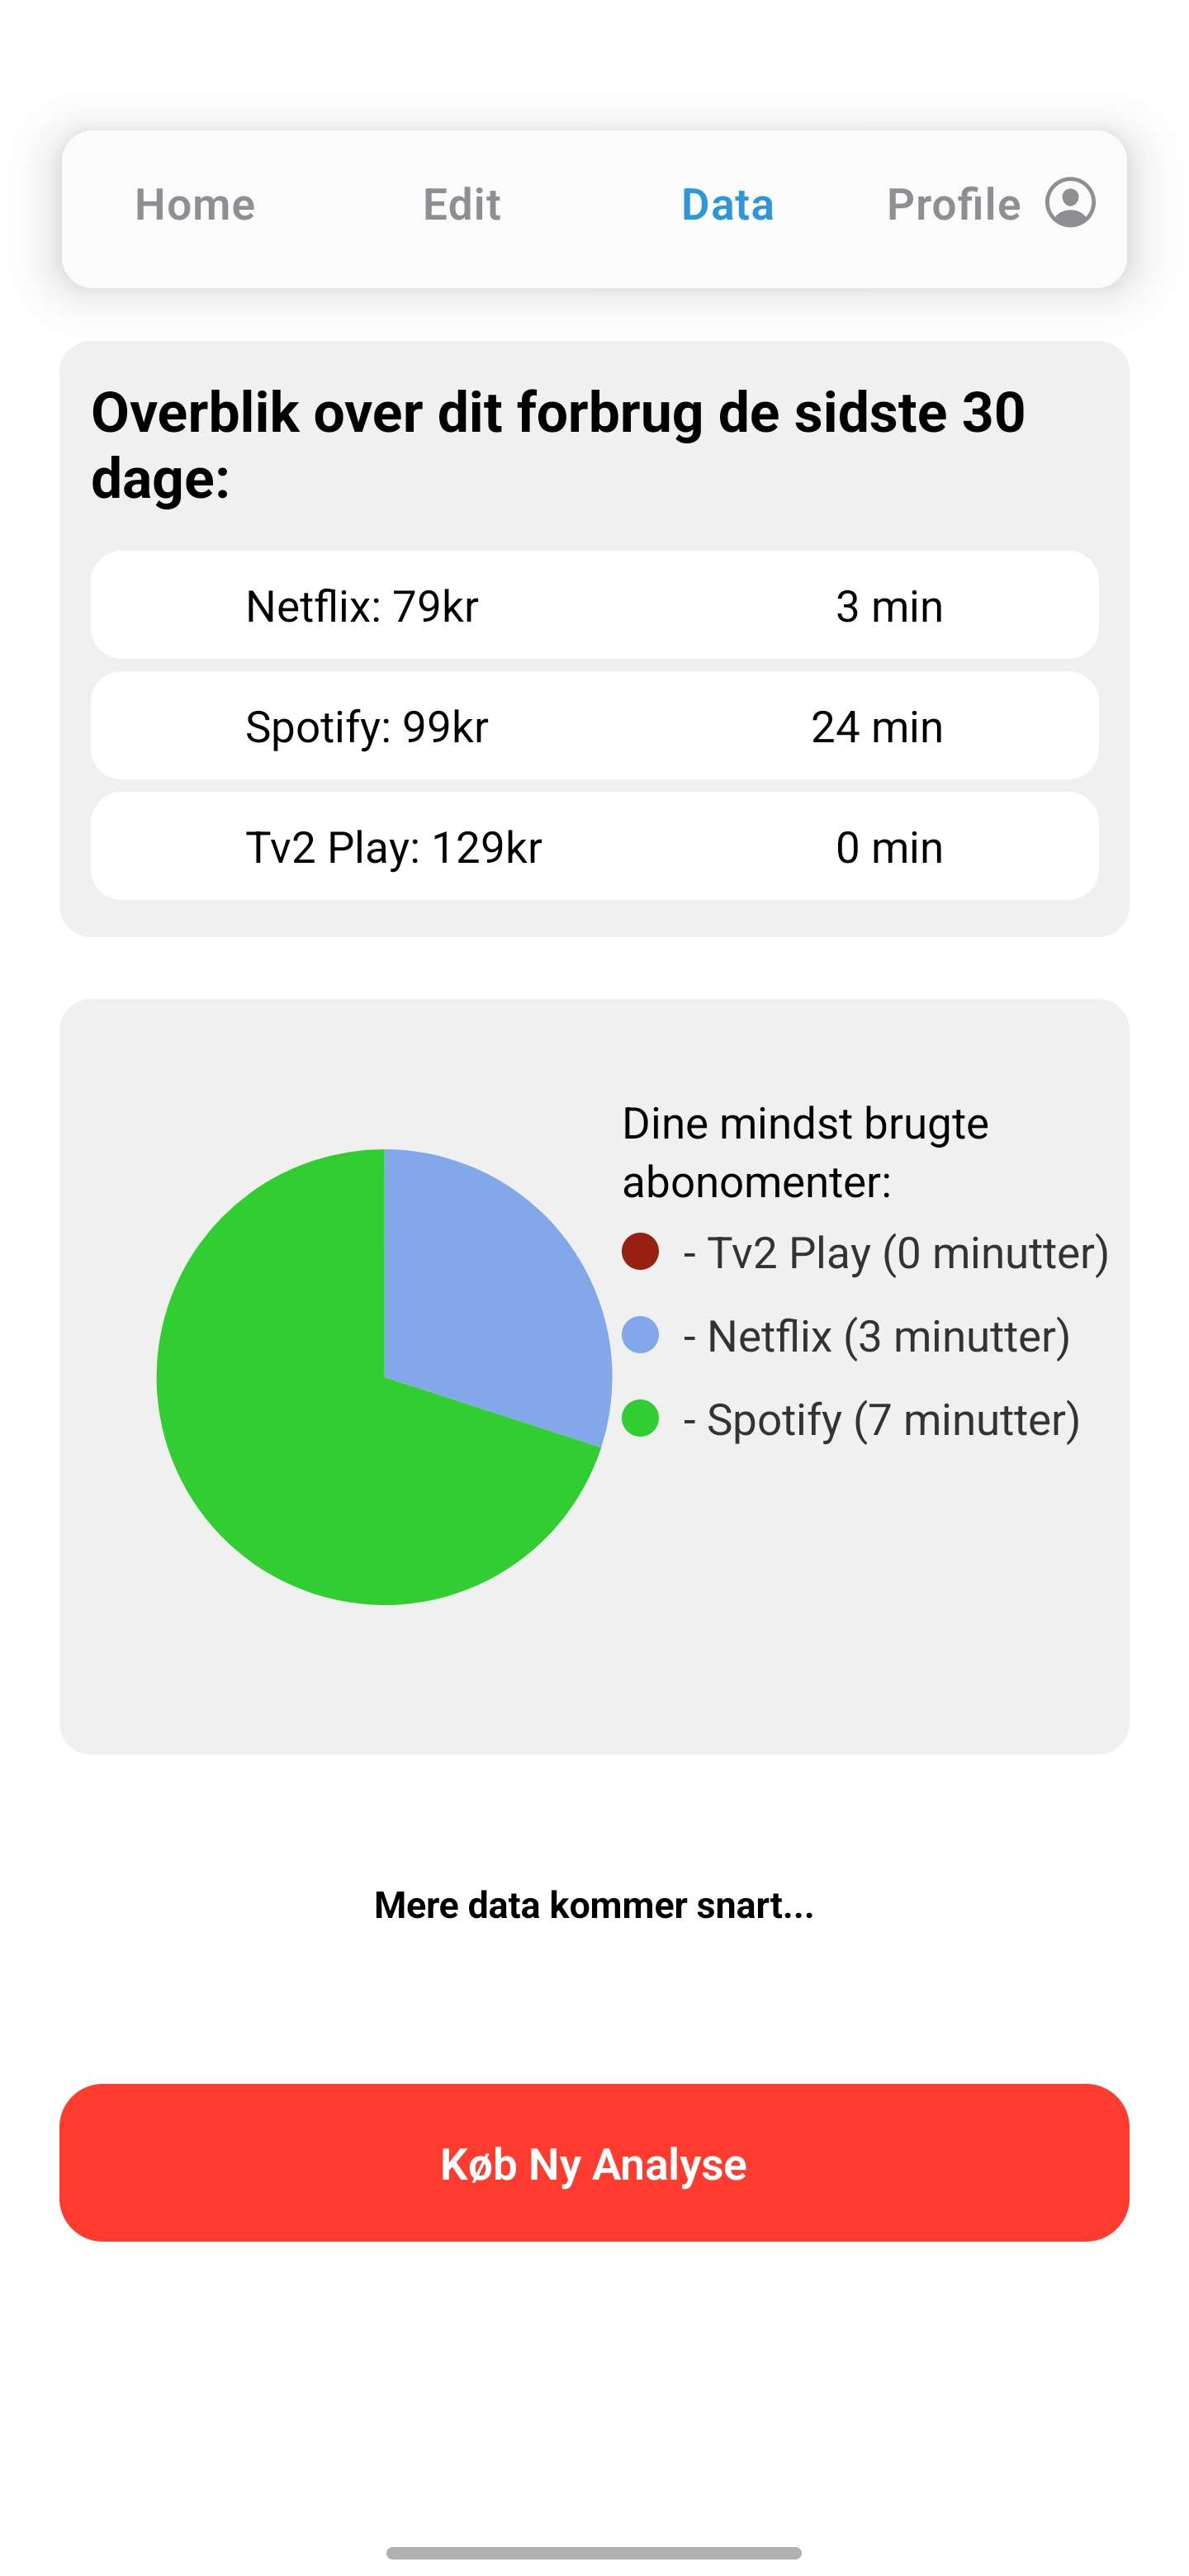
\includegraphics[width=0.5\textwidth]{assets/hifi-skitser/data.jpg}}
    \fbox{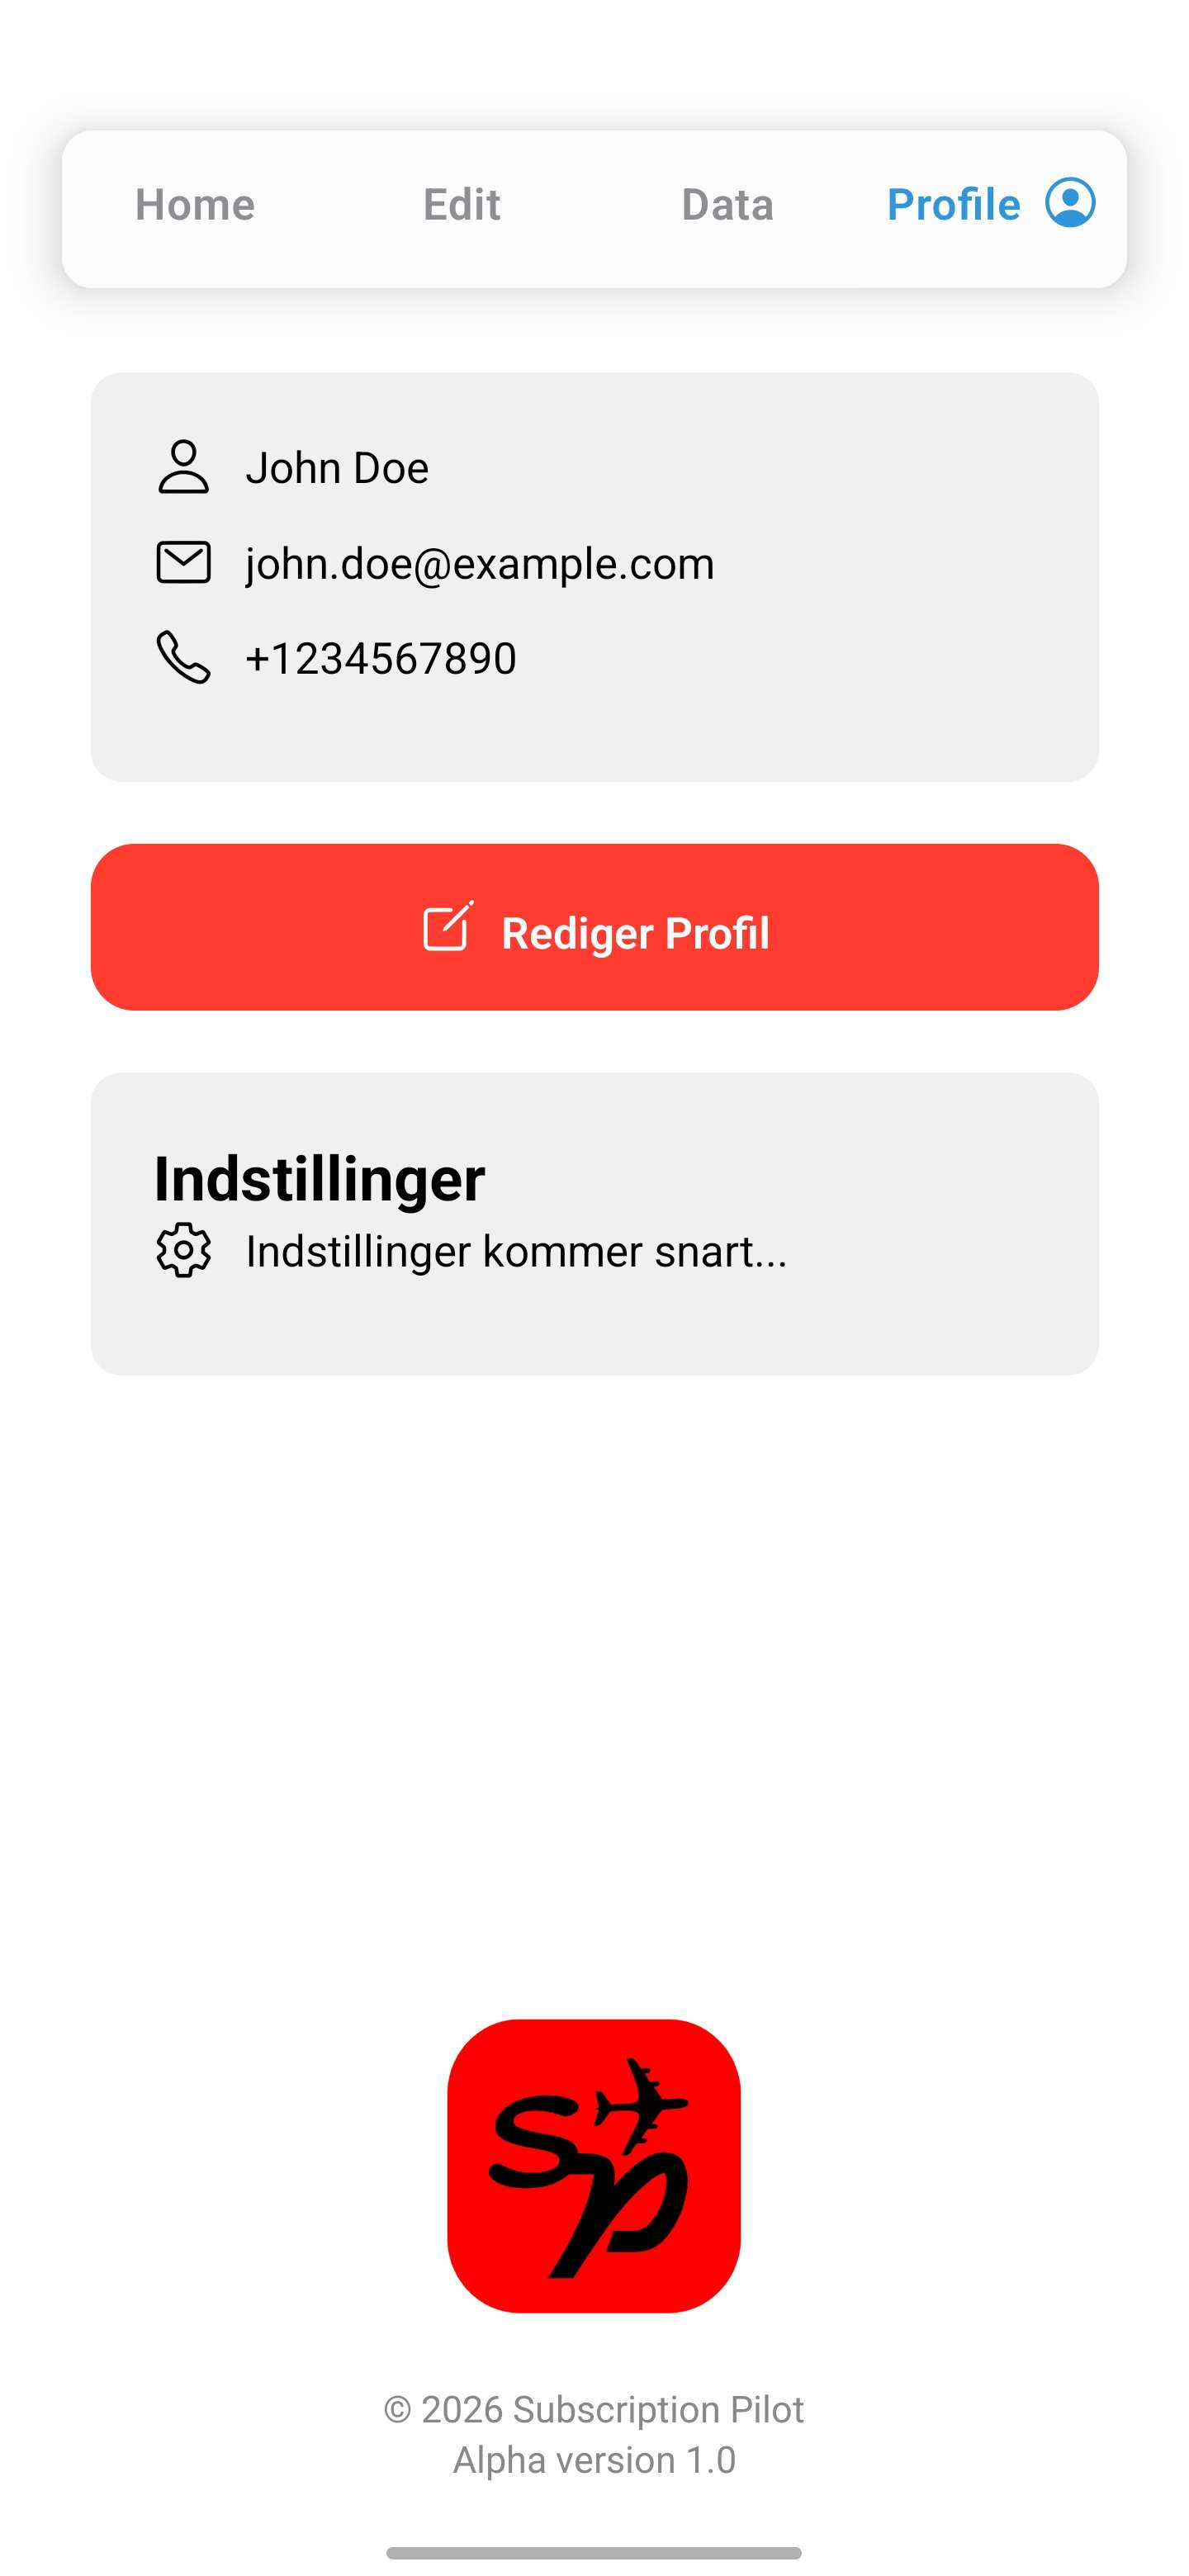
\includegraphics[width=0.5\textwidth]{assets/hifi-skitser/profile.jpg}}
  \end{figure}
\end{landscape}